\lecture{Servizi}{15~-~01~-~2026}
%
%
\section{Modelli di servizio}
I servizi rappresentano la ragione per cui il Digital Twin viene costruito. Servono a gestire le risorse, esportare predizioni e analisi, supportare le decisioni e svolgere analisi ``what-if''
%
\section{Digital Twin come DSS}
Un \gls{dss} è un sistema interattivo basato su computer che aiuta i decisori a utilizzare dati e modelli per risolvere problemi non strutturati. Unisce le risorse intellettuali degli individui con le capacità del computer per migliorare la qualità delle decisioni.

\subsection{Struttura di un DSS}
Un DSS classico combina tre componenti principali:
\begin{enumerate}
    \item Gestione dei Dati (Data Management): Raccolta, archiviazione e integrazione da diverse fonti (interne/esterne, legacy, ERP);
    \item Gestione dei Modelli (Model Management): Modelli analitici (statistici, finanziari, ingegneristici integrati con la gestione dati);
    \item Interfaccia Utente (UI): Il punto di accesso per l'utente (manager). Deve essere comprensibile e utilizzare linguaggio naturale o rappresentazioni visive;
    \item Sottosistemi basati sulla conoscenza (Knowledge-based): Supportano gli altri sottosistemi aumentando l'intelligenza (es. AI applicata ai dati).
    \item Analytics: Sviluppo di azioni basate su ragionamenti basati sulla storica dei dati (es. reports, riconoscimento pattern, predizioni).
\end{enumerate}
Vedi figura \ref{fig:servizi-dss1} a riguardo.

\begin{figure}
    \centering
    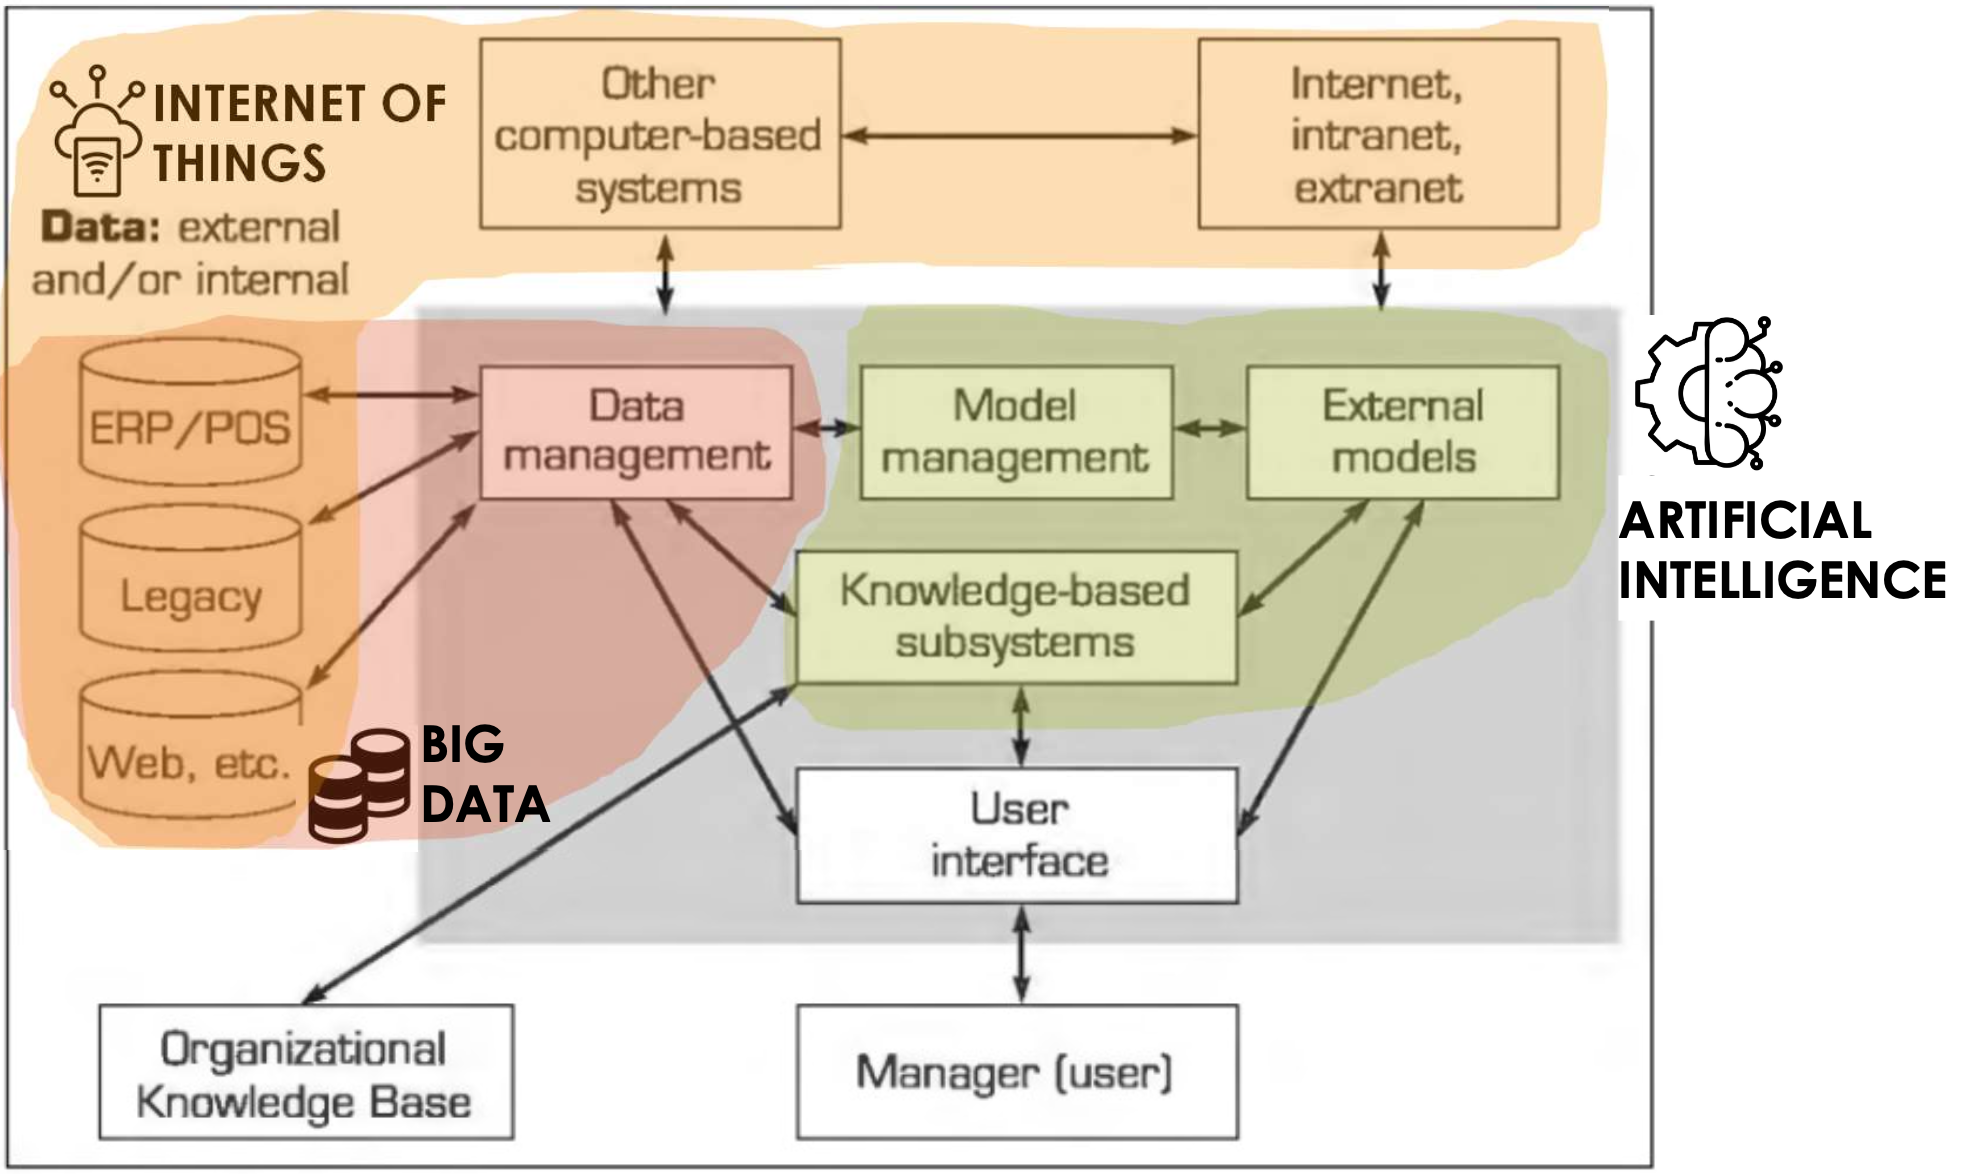
\includegraphics[width=0.7\linewidth]{assets/Screenshot 2026-01-15 at 16.52.40.png}
    \caption{Struttura di un DSS tradizionale, possiamo vedere le tre principali architetture.}\label{fig:servizi-dss1}
\end{figure}

L'architettura DSS si è evoluta verso una struttura più moderna, integrando le tecnologie dell'Industria 4.0:
\begin{itemize}
    \item Internet of Things (IoT): Nuova fonte massiva di dati esterni e interni;
    \item Big Data: Gestione di grandi volumi di dati;
    \item Intelligenza Artificiale (AI): Potenzia i sottosistemi basati sulla conoscenza.
\end{itemize}

%
\section{Service Modeling}
Ora il nostro obiettivo è definire funzioni con interfacce amichevoli per un uso ``on-demand'', rendendo meno ripida la curva di apprendimento per l'utilizzo del Digital Twin. I servizi trasformano il ``Manufacturing'' in un servizio (MaaS), permettendo la condivisione delle risorse.
%
\subsection{Classificazione dei servizi}
Tutte le risorse produttive possono essere virtualizzate e incapsulate in servizi:
\begin{enumerate}
    \item Resource Services (Servizi delle Risorse): Derivano da equipaggiamento fisico, materiali e risorse hardware;
    \item Information Services (Servizi Informativi): Risorse software come algoritmi, modelli di esperienza, conoscenza di dominio. Includono modelli di predizione, schedulazione della manutenzione, realtà aumentata e strumenti di simulazione 3D;
    \item Physical Entity Services (Servizi dell'Entità Fisica): Descrizione e stato (ID, nome, posizione), Qualità del servizio (tempo, costo), Capacità (precisione), Stato in tempo reale (in manutenzione, inattivo);
    \item Virtual Entity Services (Servizi dell'Entità Virtuale): Accessibili da più utenti contemporaneamente. Includono informazioni sul proprietario, creatore e qualità del servizio dell'entità virtuale;
    \item Data Services (Servizi Dati): Consentono l'accesso semplificato ai dati tramite template unificati (spesso in XML). I Data Services possono essere di diverso tipo, vedi figura \ref{fig:servizi-servicemodeling} a riguardo.
\end{enumerate}
\begin{figure}
    \centering
    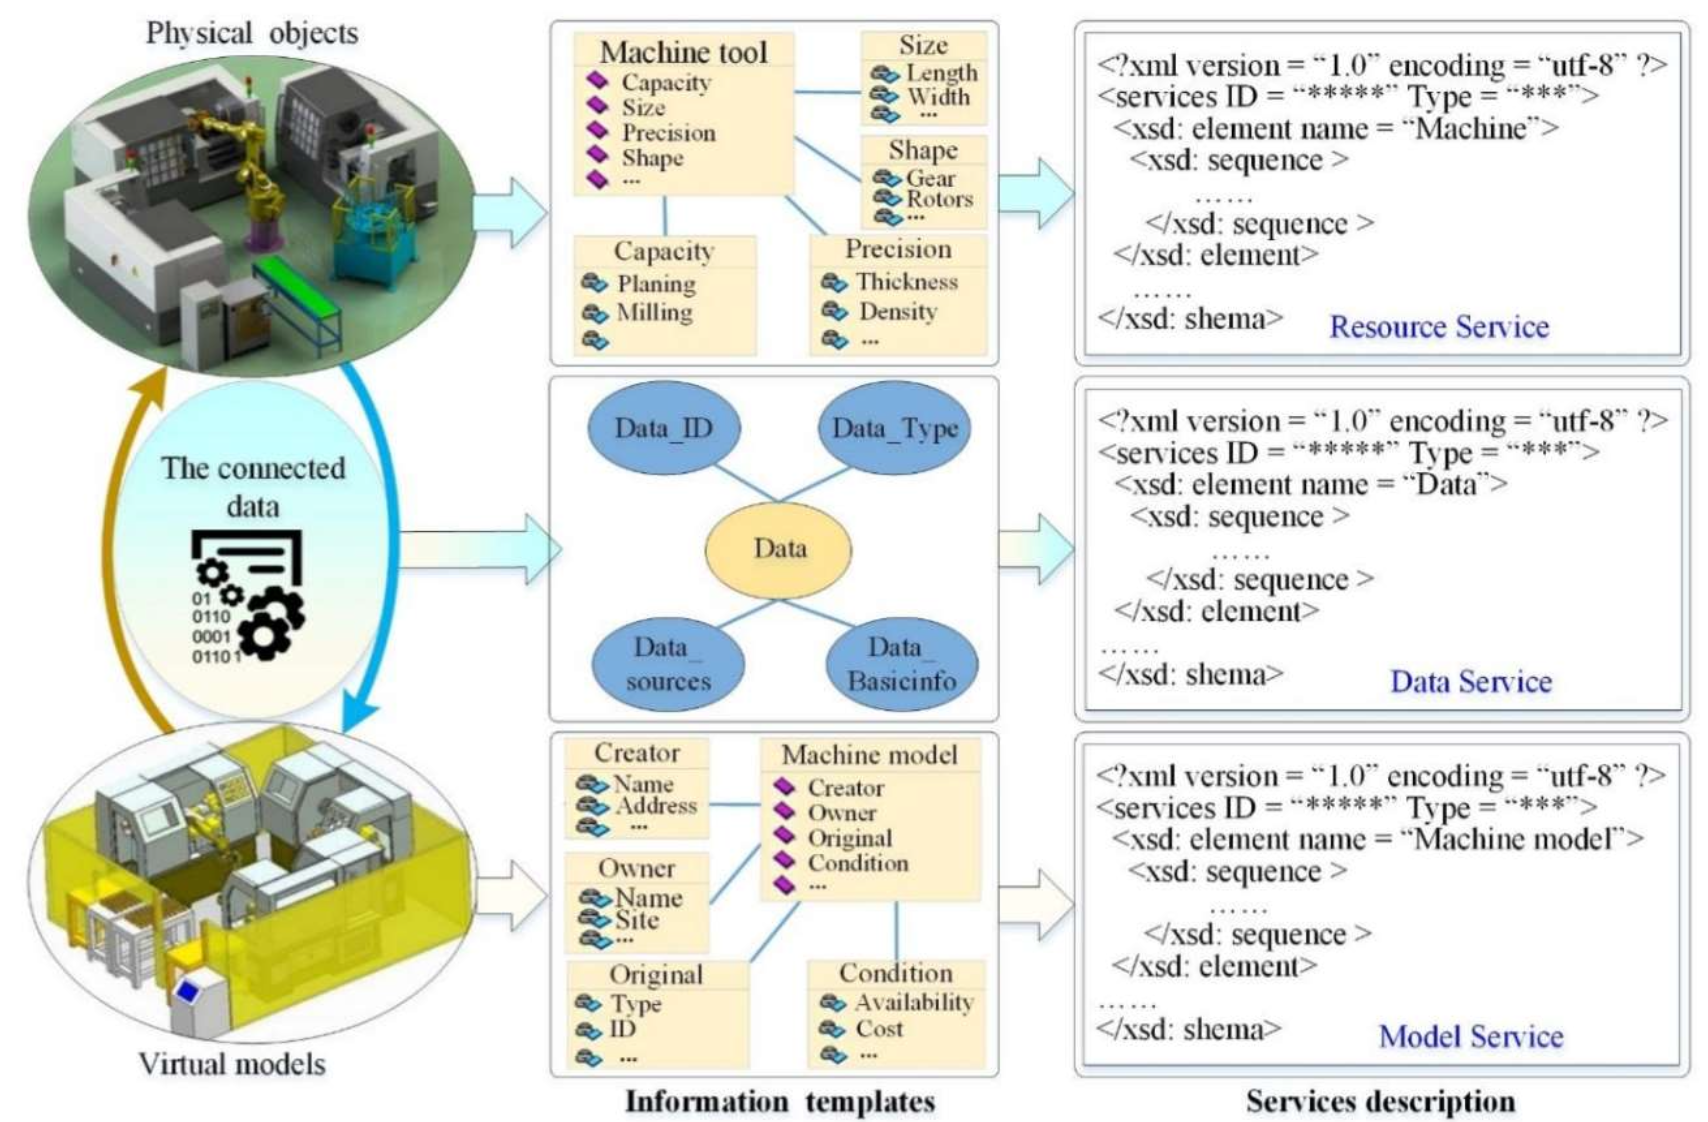
\includegraphics[width=\linewidth]{assets/Screenshot 2026-01-15 at 17.07.58.png}
    \caption{Diversi tipi di servizi di dati.}\label{fig:servizi-servicemodeling}
\end{figure}
%
\section{Dashboards}
Strumenti di gestione delle informazioni che forniscono la visualizzazioni dei dati e semplificano il ricavo delle informazioni su quest'ultimi.
%
\subsection{Grafana}
Grafana è una stack dashboard open source per l'osservabilità (metriche, log). Permette di creare dashboard per mostrare l'evoluzione dei dati e statistiche. Vedi le figure \ref{fig:dashboard-grafana-sub2}, \ref{fig:dashboard-grafana-sub3} e \ref{fig:dashboard-grafana-sub1} a riguardo.

\begin{figure}
    \centering
    \begin{subfigure}{0.6\linewidth}
        \centering
        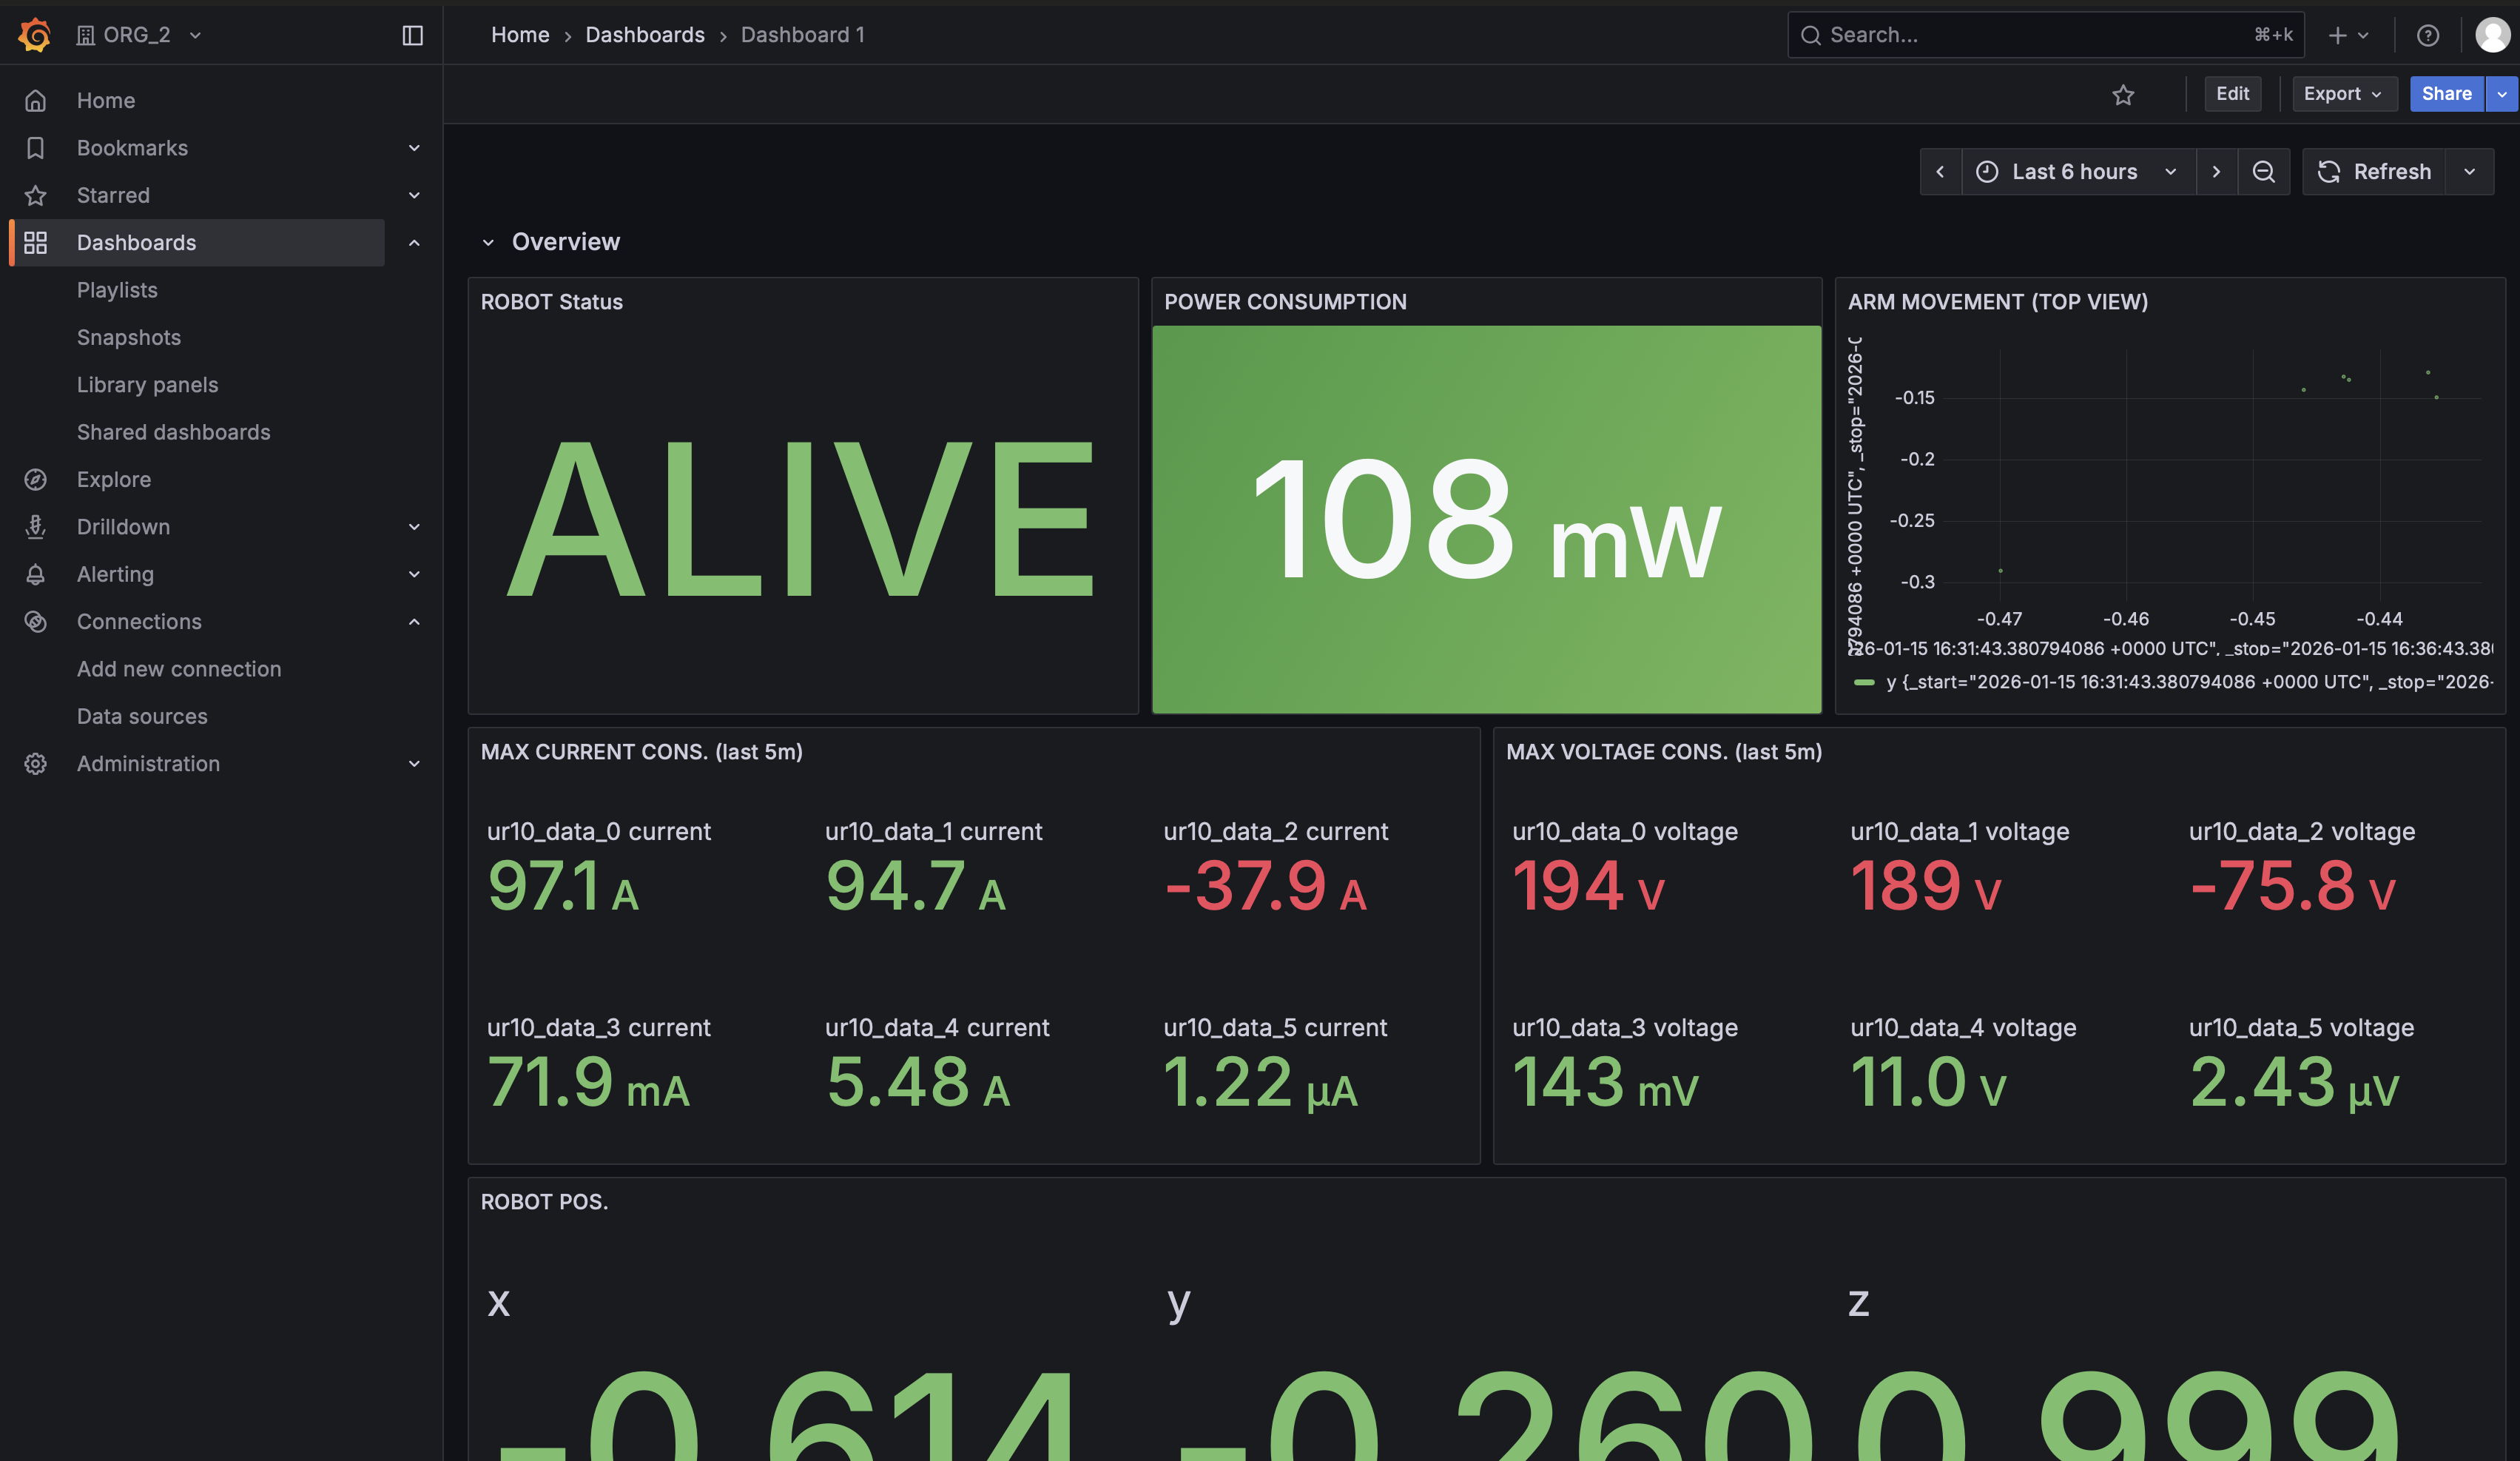
\includegraphics[width=\textwidth]{assets/Screenshot 2026-01-15 at 17.36.57.png}
        \caption{Robot Status \& Time Series Dashboard}
        \label{fig:dashboard-grafana-sub2}
    \end{subfigure}
    \begin{subfigure}{0.6\linewidth}
        \centering
        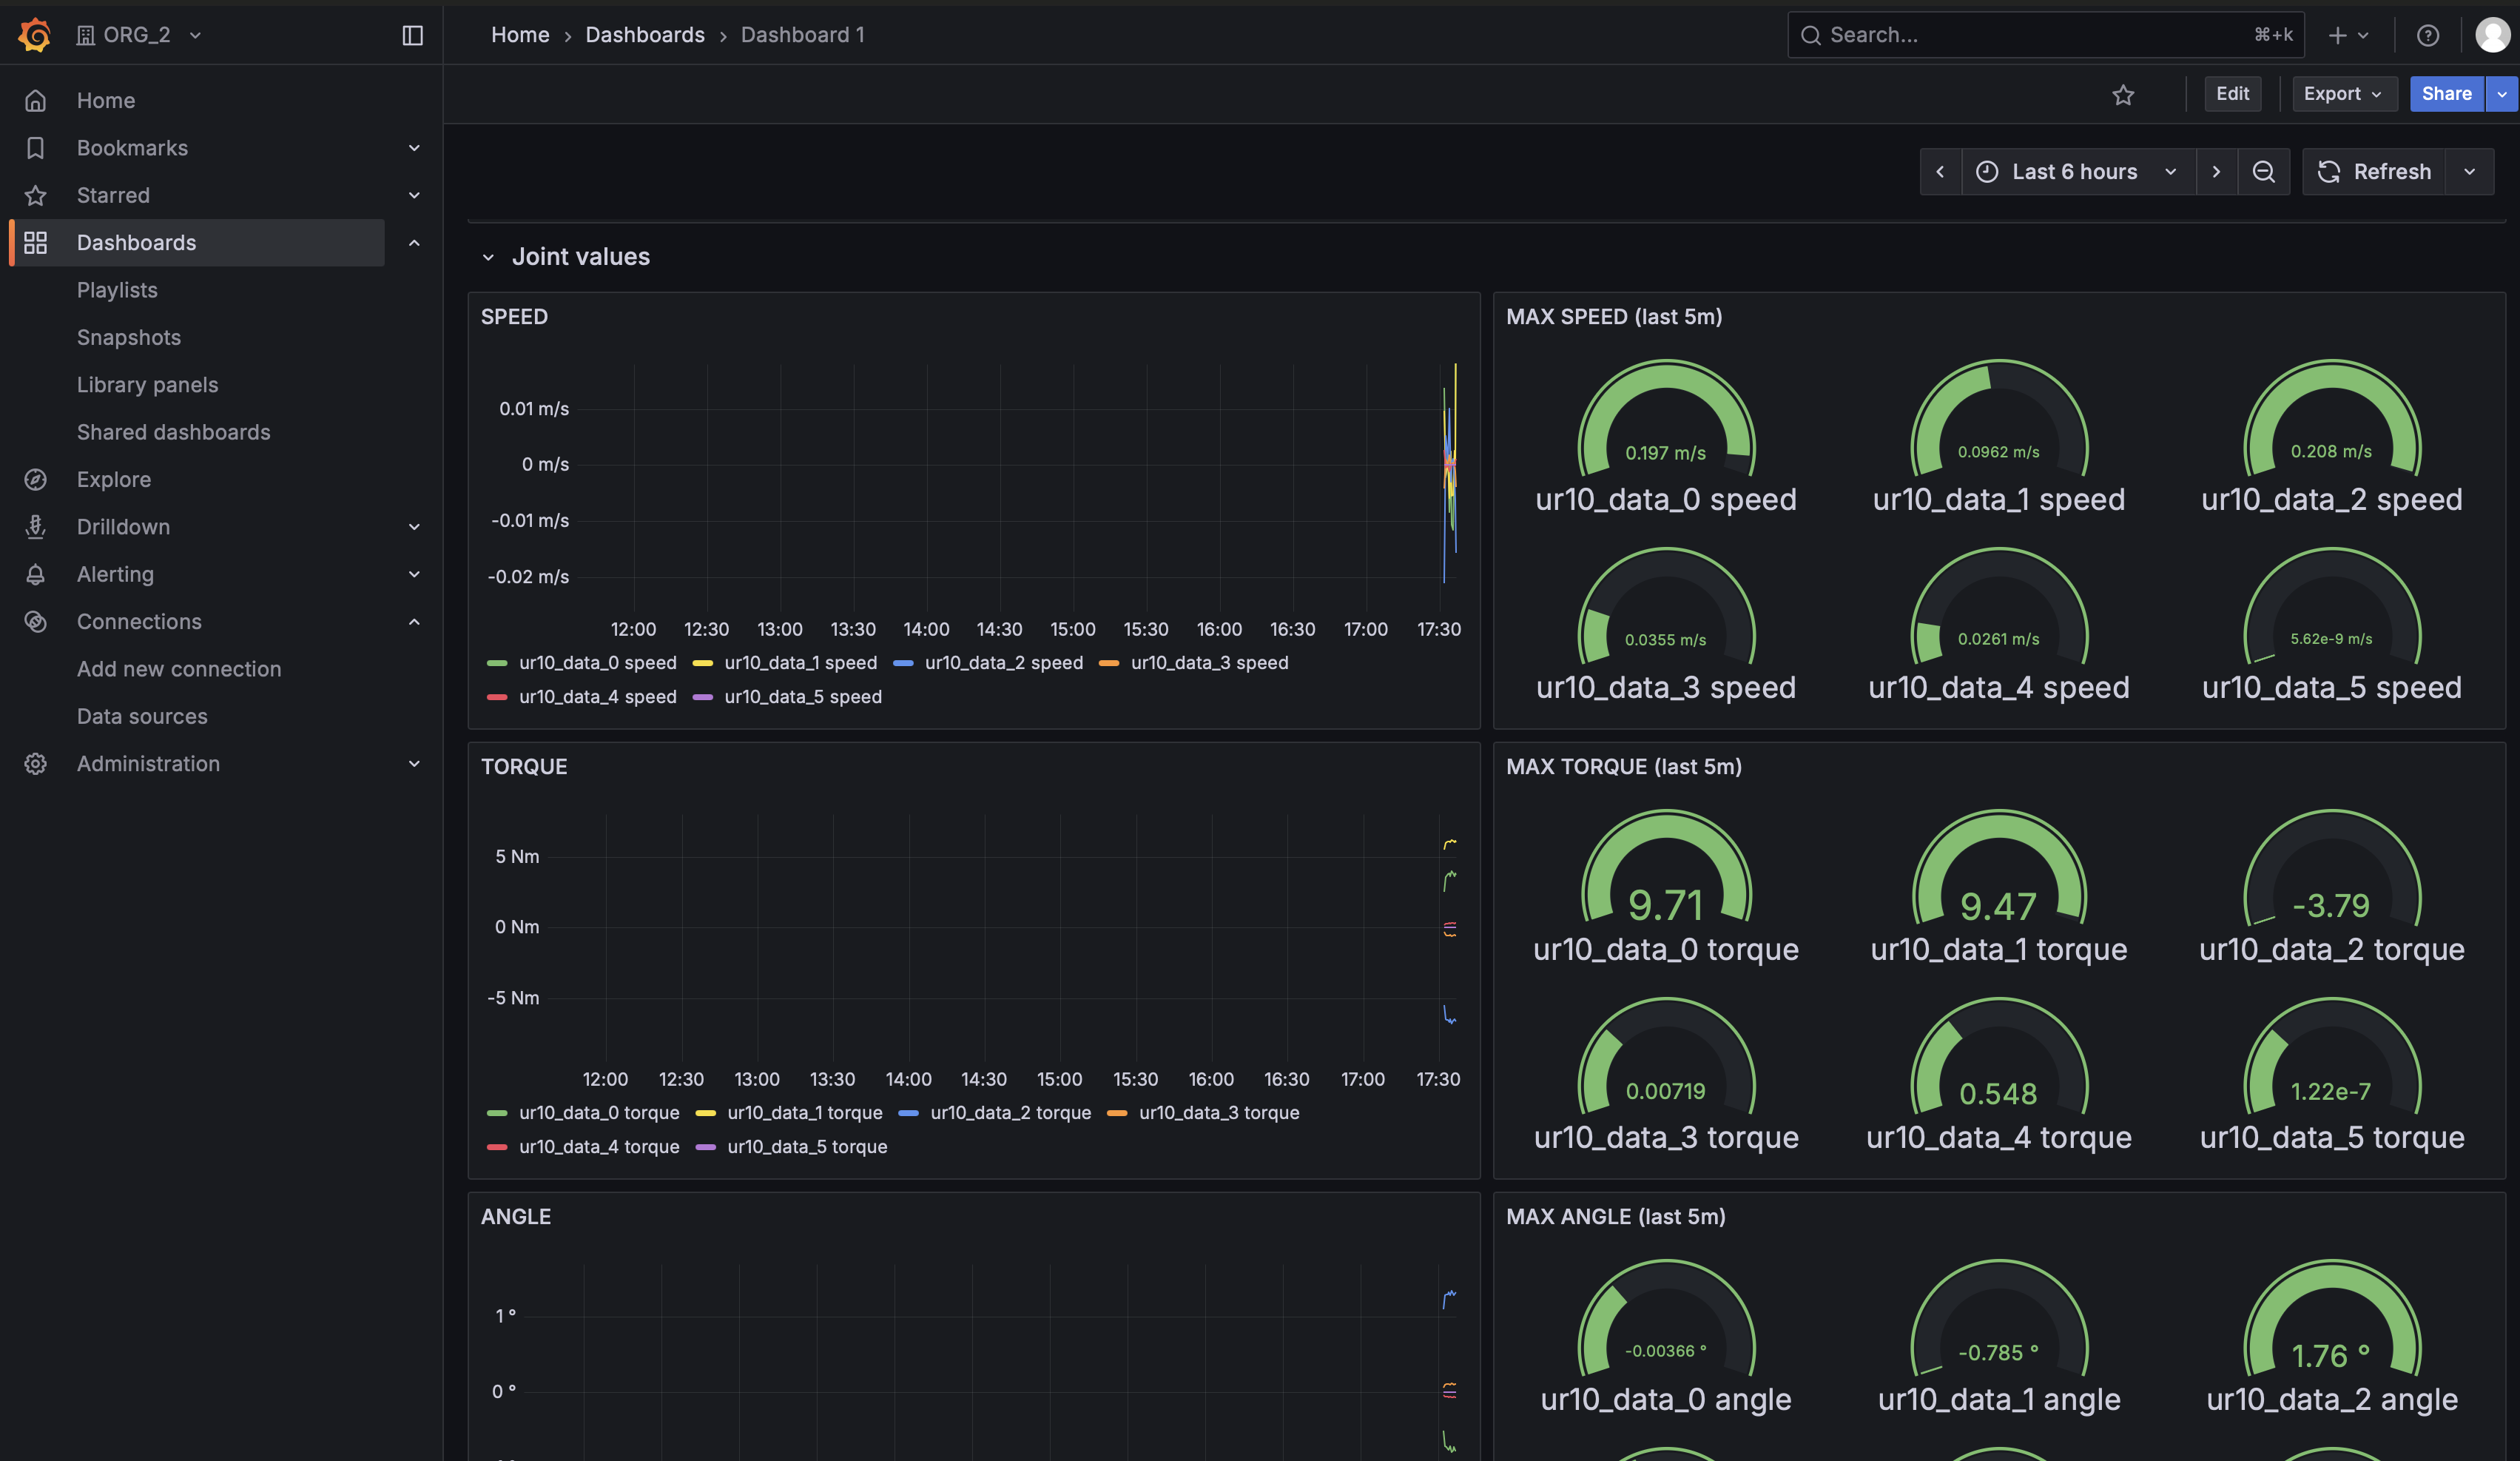
\includegraphics[width=\textwidth]{assets/Screenshot 2026-01-15 at 17.37.08.png}
        \caption{Robot Voltage Data Dashboard}
        \label{fig:dashboard-grafana-sub3}
    \end{subfigure}
    \begin{subfigure}{0.6\linewidth}
        \centering
        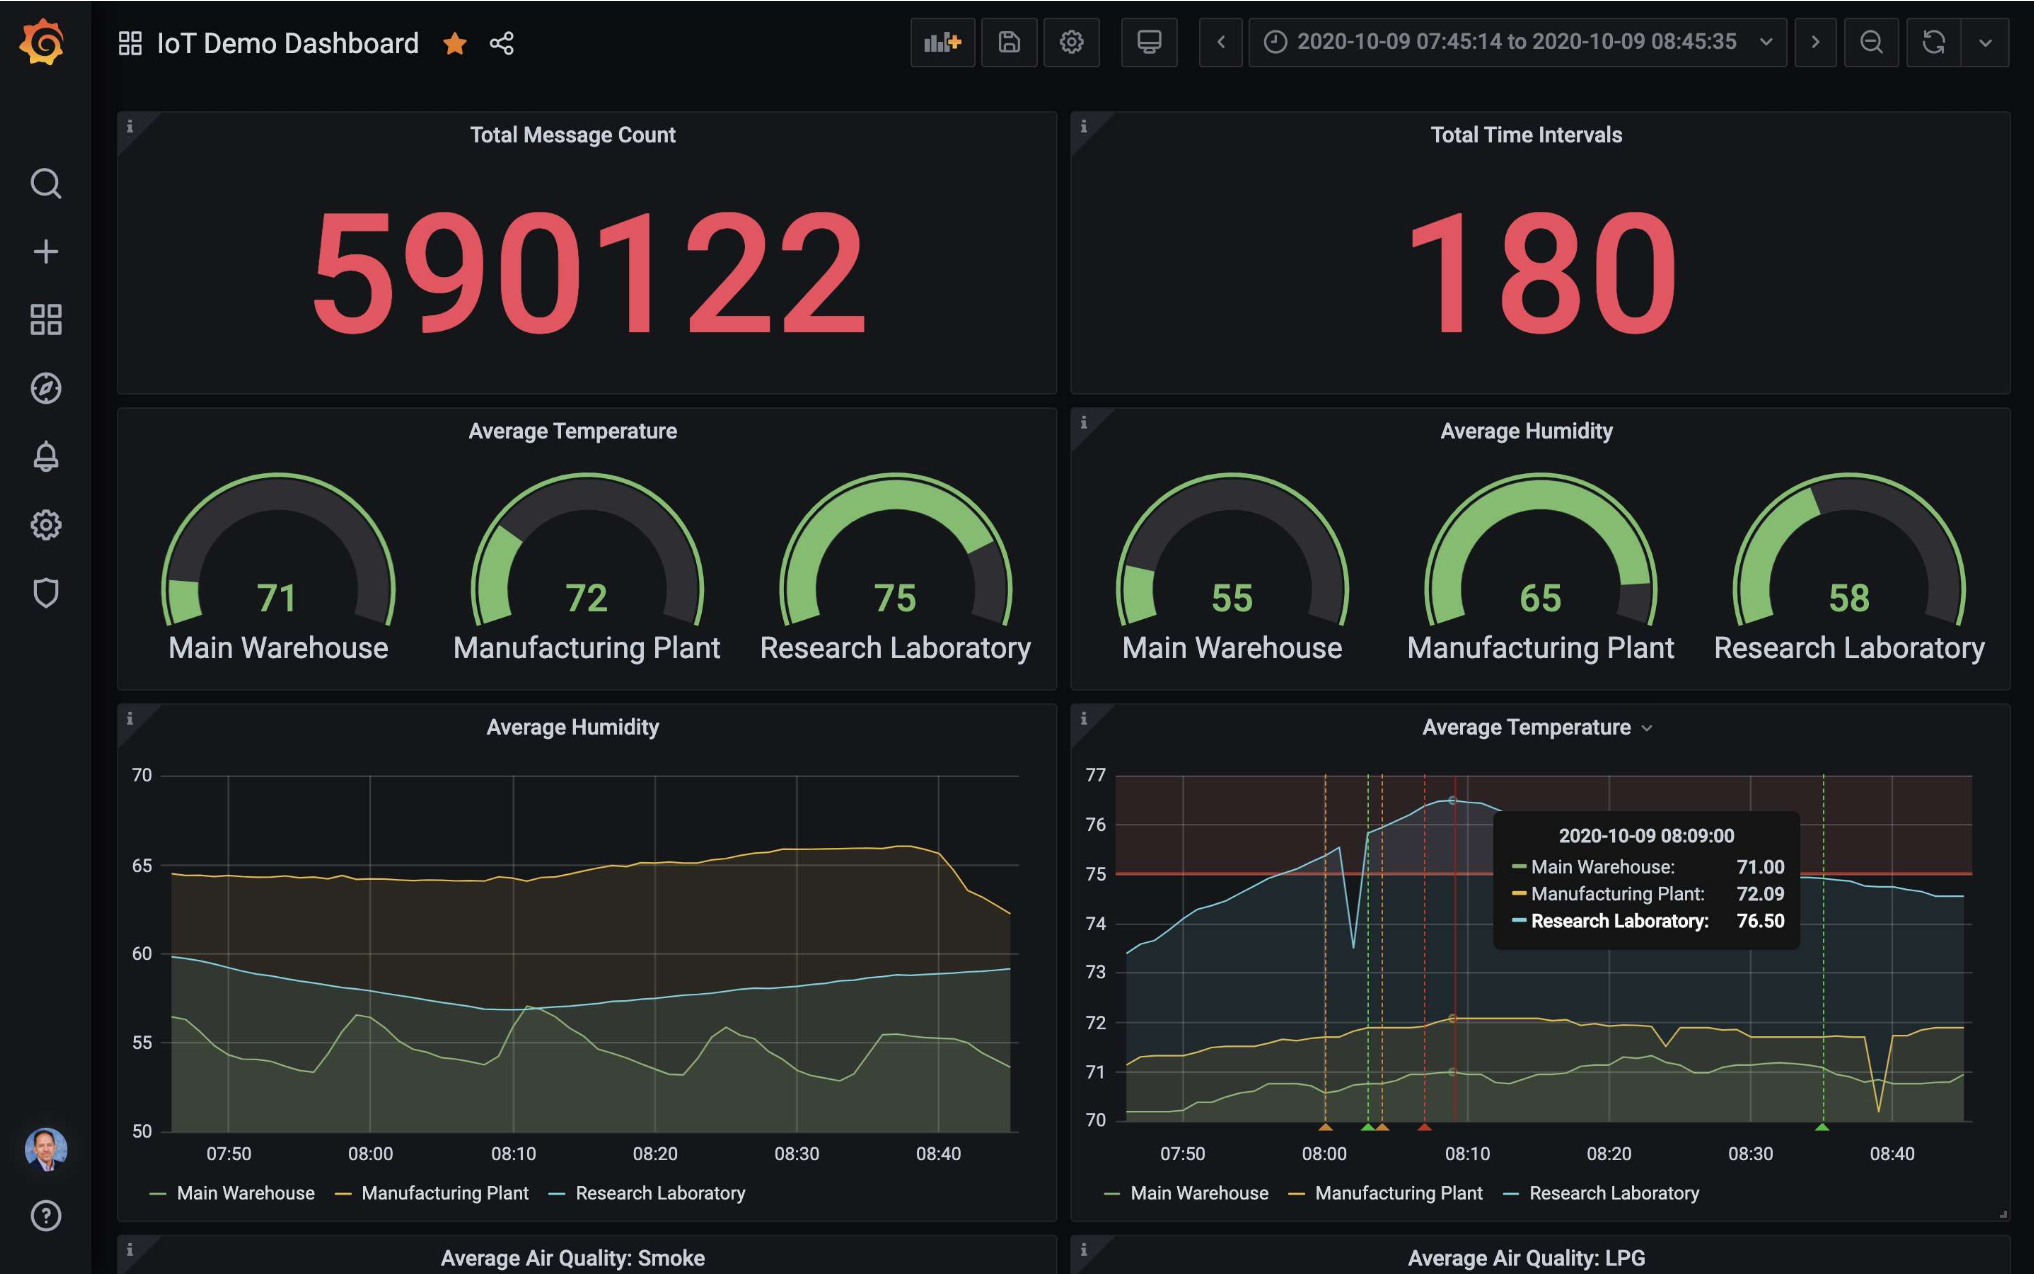
\includegraphics[width=\textwidth]{assets/Screenshot 2026-01-15 at 17.33.33.png}
        \caption{IoT Demo Dashboard}
        \label{fig:dashboard-grafana-sub1}
    \end{subfigure}

    \caption{Tre dashboard di Grafana che mostrano diversi dati.}
    \label{fig:dashboard-grafana}
\end{figure}

%
\paragraph{Flusso dei dati} ``Mondo Reale'' $ \to $ Edge Device $ \to $ Cloud Endpoint $ \to $ Time-series data store $ \to $ Motore di visualizzazione (Grafana).
